
\section{The Phase II Project}
\label{sec:phaseII}
%% {\em Provide an explicit, detailed description of the Phase I research
%%   approach and work to be performed.  Indicate what will be done, by
%%   whom (small business, subcontractors, research institution, or
%%   consultants), where it will be done, and how the work will be
%%   carried out.  If applicant is making a commercial or in-kind
%%   contribution to the project, please describe in detail here.  The
%%   Phase I effort should attempt to determine the technical feasibility
%%   of the proposed concept which, if successful, would provide a firm
%%   basis for the Phase II grant application.

%%   Relate the work plan to the objectives of the proposed project.
%%   Discuss the methods planned to achieve each objective or task
%%   explicitly and in detail.  This section should be a substantial
%%   portion of the total grant application.} 

\subsection{Technical Objectives}
%% {\em State the specific technical objectives of the Phase I effort,
%%   including the questions it will try to answer to determine the
%%   feasibility of the proposed approach.}

The requirements being addressed include the development of a robust framework 
for in-situ verification and validation in general purpose numerical simulation 
packages. In particular, the objective of this project is to address the need
for tools that automate verification of end-user numerical solutions in the 
NEAMS toolkit and workbench. 

In Phase II, RNET Technologies and ORNL will pursue the following objectives:

\begin{enumerate}

\item \rnetprop{Harden and extend the core VnV functionality developed during phase I. In particular, the phase II effort 
will look to determine the optimal approach for implementing the run time configurable test injection system such that 
the risks associated with memory corruption and constant correctness are minimized. This objective will include the miscilanious tasks
required to prepare the framework for release, including integration with a unit testing framework, futher development of the documentation generation 
engine, and documentation. }
\item \rnetprop{Develop mechanisms for efficient data movement in a distributed environment. This objective will 
look to determine and implement optimal approaches for comparing data stored in distributed arrays against an expected 
result stored on disk. The key issue here is to define approaches for describing the domain decomposition of the distributed 
array such that the experimental data can be distributed in an efficient manor. In-situ
comparison of variables with experimental and/or analytical results will be a defining feature of the framework because it significantly 
reduces the amount of IO required in \VV testing, while also providing a fine grained mechanism for detecting at what point a solution diverges from
the expected result.}
\item \rnetprop{Optimize test execution times. Initial development will focus on mechanisms for offloading tests to an external server. Offloading of tests to an
external VnV testing service has the potential to significantly reduce overall runtime. This key issue to address here 
will be to develop a mechanism for offloading data such that the data transfer is faster than simply running the test in-situ. The initial focus will be 
on determining the best framework for offloading simple tests (MRNet, SNOBall, ADIOS streaming, etc.). After that has been implemented, the focus will shift
toward implementing job based parallelism for tests the require the simulation to be run multiple times. }
\item \rnetprop{ Develop a robust set of generic \VV tests. The development of these tests (e.g., mesh refinement studies, the method of manufactured solutions, sensitivity analysis, uncertainty quantification) will further equip the users with the tools required to robustly perform end-user \VV.  The open research question the Phase II project will look to address is the optimal approach to integrating existing implementations of the tools (i.e., NIMROD, DAKOTA, MASA) into the in-situ \VV testing framework. Another open question is the development of a generic interface for mesh refinement studies such that we can automatically generate the required grid hierarchy.}
\item \rnetprop{Demonstrate the value of the VnV framework as a component in the NEAMS tools and into the NEAMS workbench. The true benefit of  
the VnV toolkit will only be realized if we can drive wide scale uptake across the entire numerical simulation community. By showing the toolkit can be used 
in the NEAMS tools, and in particular, MOOSE, libMesh and PETSc, we will demonstrate true potential of the product in libraries that are already considered 
cutting edge across the industry. Integration into the NEAMS tools will answer the NEAMS call for tools that support end-user verification
of numerical simulations. Integration into the NEAMS workbench will provide access to the tools in the seamless manor users of the workbench have come to expect. } 

\end{enumerate}

\subsection{Work Plan}
\label{sec:workplan}

As described in the objectives, the final deliverable of the Phase II project will be a fully functional, effcient, battle tested framework 
for integrating advanced end-user verification and validation into general purpose numerical simulation packages. In what follows, we outline
the work required to satisfy the objectives outlined in the previous section and to acheive these goals. 

\subsubsection{Hardening and Optimization of the Core VnV Framework}

As shown in Section~\ref{TODO}, the phase I prototype provides a simple interface that facilitates in-situ verification and validation that can be configured at runtime. In Phase II, the project team will look to address the weaknesses associated with the approach taken in Phase I; namely the system for inspecting variables in functions using (void*) pointer casts and the issues asscoiated with ensuring that the VnV tests do not alter the variables and results in any way. 

The first issue the project team will look to address will be the typecasting system for providing access to internal variables. Recall, the Phase I prototype requires the user to provide 
a list of the name and type of each variable that will be available for inspection. Under the hood, the prototype stores the ``type'' as a string, and casts the variable to a (void*). It is then the responsibility of the specfic tests to, based on the string based description of the type, ensure the pointer is cast to the correct type. The benefits of this approach are that, when implemented correctly, it is extremely eficient and that it can be compiled into any C/C++ program using any compiler. The main weakness of the approach is the reliance on the string based type specification; with the key problem being that it cannot be checked and verified during compilation. This will causes issues in cases where, say, the developer changes the type of a variable, but forgets to update the type string in the injection point.

The Phase II effort will investigate a source-code preprocessor, written using LLVM, that automatically infers the types of the variables passed to the injection points. This will be an annotation based system whereby users can mark the variables to be included at each injection point. For example, Figure~\ref{TODO} shows an example code snippet for a function with two different injection points. This will remove the need for specifying the type of each variable, ensuring the correct type is always provided to the injection point factory. It would still be up to the developer of the tests to ensure the pointer is cast to the correct state. This investgation will also include looking into using C++11 RTTI information (dynamic_cast, typeid, etc.) to infer type information at runtime; however, a general C approach will be favored due to the large number of C programs still regularly used in scientifc computing. The LLVM compiler framework will allow for fast R\&D of the pre-processor. The LLVM preprocessor will be reimplemented for use with GNU compilers at a later date. 

The second issue the Phase II effort will look to address is the requirement that VnV tests do not alter execution of the simulation in any way. While the proposed injection point system does provide some exciting opportunities for run-time computational steering and parallel debugging, the framework will be, first and foremost, designed for \VV, and as such, there needs to be an option to verify the constant correctness of each test.

In Phase II, we will implement a constant correctness system based on ideas borrowed from relative parallel bebuggers. In these cases, the idea is to

\subsubsection{Reducing Runtimes with Test Offloading and Job Parallelism}


\subsubsection{Efficient Statistical Comparrisons in Distributed Settings}


\subsubsection{Generic \VV tools for Mesh Refinement, Uncertainty Quantificaiton and Sensitivity Analysis.} 

\subsubsection{Demonstration in Real World Applications}


\subsubsection{Integration with the NEAMS workbench} 







\subsection{Performance Schedule and Task Plan}
\label{sec:taskplan}

% Use wrapfigure here instead?
\begin{wrapfigure}{r}{0.5\linewidth}%[thb]
%\begin{figure}[thb]
\begin{center}
\leavevmode
%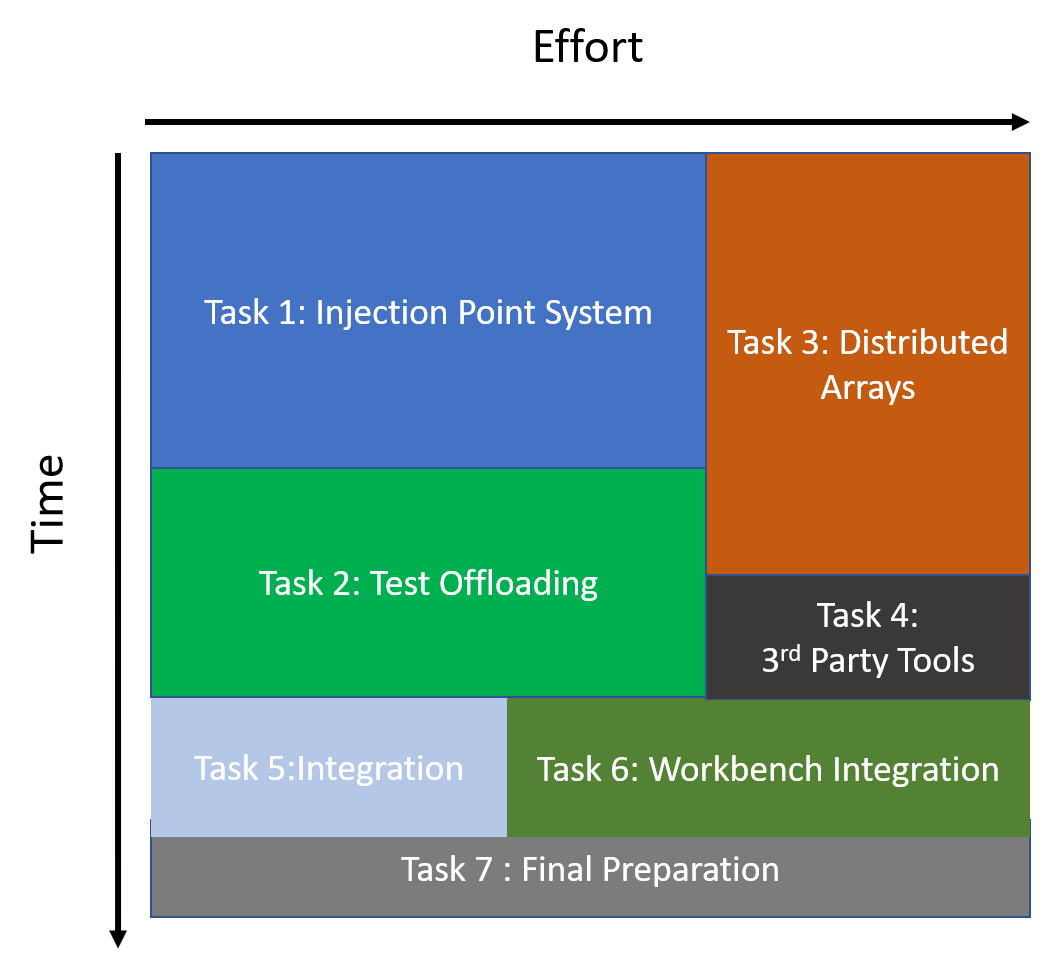
\includegraphics[width=1.0\linewidth]{./narrative/figures/tasks.pdf}
\end{center}
\caption{Overview of task dependencies and timeline.}
\label{fig:tasks}
\end{wrapfigure}

RNET would like to present the project ideas and research plan to the
DOE Program Manager and other interested scientists. The meeting will
be used to discuss features, and identify the specific NEAMS applications and computer
resources that will benefit from this project.  This meeting will be
scheduled soon after the Phase II contract is awarded. The meeting can
be hosted at RNET, a DOE site suggested by the Program Manager or via
a teleconference.

RNET will submit all reports as required by the contract (e.g., annual reports, 
a continuation report, summary reports, and a final report) to the DOE program 
manager and other interested DOE scientists.

The research and development topics described in Section~\ref{sec:workplan} 
will be addressed by the tasks described in the remainder of this section. Most 
tasks require active collaboration between RNET and its collaborators. 
Figure~\ref{fig:tasks} summarizes at a high level the dependencies among tasks  and
approximate anticipated task durations. The duration of the Phase II 
project is 104 weeks. Specific details are included in the description of each 
task.


\newcounter{taskCount}
\setcounter{taskCount}{0}

\refstepcounter{taskCount}\label{task:2.5}
\subsubsection{Task \ref{task:2.5}: Hardening of the Phase I VnV Injection Point System. }

In this task, the project team will develop an efficient, intuitive and type-safe injection point system for specifying testing points in, and across, advanced numerical software packages. Building on top of the Phase I prototype, this work will look to implement the injection point system in a way that allows for in-situ variable inspection in a robust and consistent way. The two main that need to be addressed are (1) the distinct lack of a robust reflection API in C++ makes defining functions that support generic arguments of unknown classes in a type safe way difficult, (2) the overhead associated with \VV injection points in cases where no testing is requested and (3) the difficulties in ensuring tests do not modify the variables in any way. Implementing this will require looking into the possibilities of implementing a LLVM compiler option for run-time removal of unused injection points, and/or the development of binary rewriting tools and the integration of parallel relative debugging techniques for detecting un-authorized and/or unintended changes is the run-time variables. 

\rnetprop{RNET will work on the implementation for this task and ORNL will provide inputs and guidance.}


\refstepcounter{taskCount}\label{task:3}
\subsubsection{Task \ref{task:3}: Develop methods for offloading tests to external processes. }
Performing a large number of \VV tests in a distributed environment will be expensive, both computationally and due to the data movement required to deal with the domain decomposition employed by the application. In this task, the project team will investigate the development of a mechanism for the evaluation of \VV tests that is lightweight and minimizes resource consumption. The initial approach to this will be to determine the requirements for efficient \VV test execution, and assess the capabilities provided by frameworks such as MRNet, SNOflake, ADIOS, etc. to determine if they can meet these requirements. Depending on the results of this assessment, work will be undertaken to create a library that can be integrated with the \VV framework. This library will be based on either one of these frameworks or using a custom solution. The project team will also determine the feasibility of integrating the Parallel Tools Platform (PTP) as a mechanism for minimizing \VV runtime through job parallelism. If appropriate, the team will extending PTP to fit this purpose.   

\rnetprop{RNET will work on the implementation for this task and ORNL will provide inputs and guidance.}

\refstepcounter{taskCount}\label{task:23}
\subsubsection{Task \ref{task:23}: Development of efficient statistical \VV tools with a focus of performance in large scale distributed settings.}

In this task, the team will perform R\&D work to determine and implement efficient statistical based \VV tools that can be applied in distributed settings. Consider that case of comparing the simulated solution to some known experimental results. In a distributed setting, the user must either distribute the experimental data across the nodes based on some known description of the data decomposition (difficult in a general setting), or gather to solution to some root node (expensive, and in many cases impossible. In this task, the project team will look into efficient mechanisms for inferring, detecting, and or describing the data decomposition such that this style of tests can be completed in an efficient manner. 

\rnetprop{RNET will be responsible for this task. ORNL will provide guidance on 
developing the framework for ORNL CADES.}

\refstepcounter{taskCount}\label{task:22}
\subsubsection{Task \ref{task:22}: Development of Generic tools for Mesh refinement, Uncertainty quantification and Sensitivity Analysis.}
In this task, RNET will implement generic \VV tools for mesh refinement, uncertainty quantification and sensitivity analysis. In the case of mesh refinement, the approach taken will be to create a generic interface for interacting with the automatic mesh refinement functionality that already exists in finite element libraries like LibMesh and Fenics. The overall goal is to create a generic VnV test that can be attached to the main function of the executable such that it automates the process of running mesh refinement and mesh convergence studies. In the case of UQ and SA, the project team will develop an interface for specifying the tools available in DAKOTA as VnV tests. 

\rnetprop{RNET will be responsible for this task. ORNL will provide guidance on 
developing the framework for ORNL CADES.}


\refstepcounter{taskCount}\label{task:4}
\subsubsection{Task \ref{task:4}: Extension of the VnV report generation system}
In this task, the project team will complete the development of the VnV report generation system. he primary goal of this task will be
to provide support for generating VnV reports that conform to the specification outlined in the DoD VV report templates.  The task will also include  a full implementation 
of the VnV markdown extension to support a wide variety of data visualization components, the development of the interfaces required for displaying unit and regression testing
reports, and the software indirections required for assimilating multiple VnV reports into a single document that can be used in the \VV of an entire simulation package. 

\rnetprop{RNET will work on the implementation for this task}

\refstepcounter{taskCount}\label{task:1}
\subsubsection{Task \ref{task:1}: Integration into real applications, including the NEAMS Tools}
\rnetprop{
  In this task, the program team will integrate the VnV framework into a variety of real applications. Initially, this 
  testing will be completed in tools used heavily in the NEAMS toolkit; MOOSE, libMesh and PETSc, but other third party 
  applications will also be investigated. To ensure seamless integration with the MOOSE tools, the project team will reimplement
  the XML based configuration file using the MOOSE input file format. This will allow for the configuration of the VnV tests in 
  a MOOSE application directly from the input file.
  
  The goal of this task will be to generate informative, production quality VnV 
  reports for a number of examples available in the MOOSE testing suite. Doing so allows us
  to test every facet of the proposed framework, while also acting the first demonstration of the
  value provided by the framework. These results of these tests will be hosted on the RNET website 
  as they become available. 
 

}

\rnetprop{
RNET will be responsible for this task and ORNL will provide guidance on 
various technical implementations and details.
}
\refstepcounter{taskCount}\label{task:11}
\subsubsection{Task \ref{task:11}: Development of an interface for the NEAMS workbench}
\rnetprop{
  In this task, the project team will integrate the toolkit directly into the NEAMS workbench. This will be
  a two stage process. First, the project team will implement the required interface files for enabling 
  the context aware auto-complete features available in the NEAMS workbench for the MOOSE based configuration
  file specification developed in the previous section. MOOSE based input files are already largely supported in
  the workbench; however, there will likely be some issues with determining which tests are applicable at which 
  injection points. Second will be developing an interface for customizing and viewing the final VV report. As part of the Phase I
  effort, the project team demonstrated viewing the final \VV report in a QT WebView component. The workbench is also but on to
  off QT, hence we do not expect to many difficulties on that front. Instead the key objective will be to develop the mechanisms for
  displaying customizations made the the final report in real-time within the NEAMS workbench. 
}
\rnetprop{ RNET will be responsible for this task }


\subsection{Facilities/Equipment}
\subsubsection{RNET Facilities}
RNET has the necessary office equipment to manage an SBIR/STTR contract
including networks, workstations, and accounting software. In
addition, RNET has the tools (software and hardware) to evaluate and
develop the technologies proposed here.  

RNET currently has 9 development computers and a 10-node development cluster 
that can be used for development and testing in this effort. Each cluster node 
has two quad-core or hexa-core XEON CPUs, 24-32GB of DRAM, 500+GB of local 
disk. 
Two data networks are available, a COTS 1 Gbps Ethernet network and a 10 Gbps 
Ethernet network. The Linux development nodes and the RNET cluster have the 
necessary Linux/GNU toolchains and development environments including; GNU 
tool chain, Microsoft .Net Framework, and Java Standard Edition.

\subsubsection{ORNL Facilities}
%\rnetcomment{Jay to verify, can we state these resources can be used on this project?}
The Oak Ridge National Laboratory (ORNL) hosts three petascale computing 
facilities: the Oak Ridge Leadership Computing 
Facility (OLCF), managed for DOE; the National Institute for Computational 
Sciences (NICS) computing facility operated 
for the National Science Foundation (NSF); and the National Climate-Computing 
Research Center (NCRC), formed as 
collaboration between ORNL and the National Oceanographic and Atmospheric 
Administration (NOAA) to explore a variety of 
research topics in climate sciences. Each of these facilities has a 
professional, experienced operational and engineering 
staff comprising groups in high-performance computing (HPC) operations, 
technology integration, user services, scientific 
computing, and application performance tools.

%\rnetcomment{Ram: Based on Jay's comments.}
ORNL also has the Compute and Data Environment for Science (CADES) which is a 
fully integrated infrastructure offering compute and data services for 
researchers lab-wide. We will work with appropriate program managers to apply 
for allocation requests as appropriate.


 The ORNL computer facility staff 
provides continuous operation of the centers 
and immediate problem resolution. On evenings and weekends, operators provide 
first-line problem resolution for users with 
additional user support and system administrators on-call for more difficult 
problems. ORNL also has state-of-the-art 
visualization facilities that can be used on site or accessed remotely. 
